\documentclass[a4paper]{article}     
\usepackage{amsfonts}
\usepackage{amsmath}
\usepackage{amssymb}
\usepackage{graphicx}

\newcommand{\dint}{\displaystyle\int}

\begin{document}

\noindent \large Auteur: Mark Gijsbrechts \\
\noindent \large Studierichting: Informatica\\
\noindent \large Oefeningenreeks 5K nr. 1.1\\

\medskip

\normalsize





$ r = 2 \cos \theta $ \\

$ r^2 = 4 \cos^2 \theta $ \\

$ r' = -2 \sin \theta \Rightarrow (r')^2 = 4 \sin^2 \theta $ \\

$ L = \dint_{-\tfrac{\pi}{2}}^{\tfrac{\pi}{2}} \sqrt{4\cos^2 \theta + 4\sin^2 \theta} d\theta $ \\

$= \dint_{-\tfrac{\pi}{2}}^{\tfrac{\pi}{2}} \sqrt{4 \left( \cos^2 \theta + sin^2 \theta \right)} d\theta $ \\

$= \dint_{-\tfrac{\pi}{2}}^{\tfrac{\pi}{2}} \sqrt{4} d\theta $ \\

$= 2 \dint_{-\tfrac{\pi}{2}}^{\tfrac{\pi}{2}} d\theta $ \\

$= 2 \left[ \theta \right]_{-\tfrac{\pi}{2}}^{\tfrac{\pi}{2}} $ \\

$= 2 \left[ \dfrac{\pi}{2} - \left( - \dfrac{\pi}{2} \right) \right] $ \\

$= 2 \pi $ \\


\begin{figure}[h]
\centering
    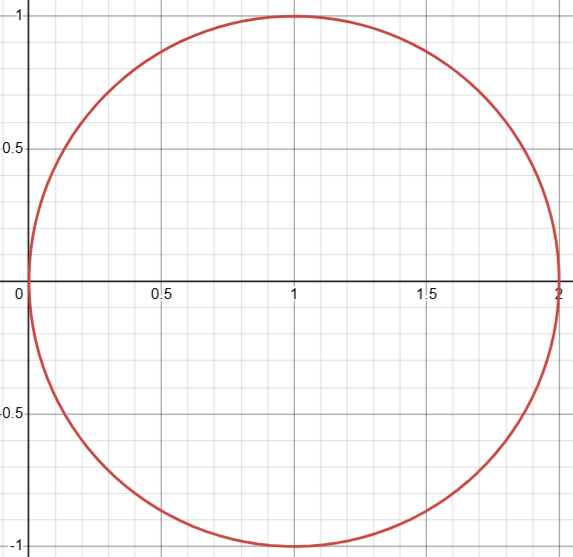
\includegraphics[width=\linewidth]{5K-1.1-mark.gijsbrechts.INF.png}
\end{figure}




\begin{thebibliography}{999}
%\bibitem{a} Referentie
\end{thebibliography}
\end{document} 
